\section{Graph Conversion}\label{sec:conversion}

As stated in Section \ref{sec:graph-representation}, many different approaches for graph conversions have been proposed. Our approach is inspired by that of Boisvert et al. \cite{boisvert2024towards}, but, unlike them, we do not include domain values in our representation. We decided to exclude domain values for practical reasons: the argument of Boisvert et al. to include them, lies on the injection of the conversion, without domain values two instances could end up being mapped into the same graph. While true, our primary objective is to use the features for algorithm selection and, as an example, an instance from the 2025 Minizinc challenge\footnote{\url{https://www.minizinc.org/challenge/2025/results/}} (coming from the cgt problem with instance name cgt\_12\_h27\_r0.05\_s0.5\_3) had an objective function with a domain between -1.932.060 and 1.714.644, resulting in 3.646.705 total possible values just for one domain. The full instance would also require adding also other variables and their domains as well as constraints and operators. A graph with this many nodes would be intractable for our purposes. Furthermore, our graphs are directed instead of undirected. This choice allow us to have shallow graphs with small diameters making it possible to convey all the information with a limited amount of aggregation steps. We have decided to use Boisvert et al.'s syntax tree-like representation as it allows us to decompose complex constraints into simpler elements that could be reused in different constraints with similar meanings.

In more details, we define five types of nodes:
\begin{itemize}
    \item \textbf{Variable nodes}: representing the variables of the problem. 
    \item \textbf{Solution node}: a single node for each problem that represents the type of problem (Minimisation, Maximisation or Satisfaction).
    \item \textbf{Parameter/Literal nodes}: representing the literal values of the problem (e.g. 1, 2, True, False, etc.).
    \item \textbf{Operator nodes}: representing arithmetic and functional operations between variables, parameters and other operators (e.g. $+$, $\times$, $\div$ etc.) Operator nodes have a sub-category for the type of operator represented.
    \item \textbf{Constraint nodes}: representing relational predicates (e.g. $=$, $\neq$, $<$, $\leq$), logical operations (e.g. $\wedge$, $\vee$, $\neg$), and global constraints (e.g. \texttt{all\_different}, \texttt{table}). Constraint nodes also have a sub-category for the type of constraint the node represents. 
\end{itemize}
All node and sub-node types we have defined for the conversion from FlatZinc can be seen in the Appendix \ref{sec:node-types}.

As previously mentioned, edges between nodes are directed: variables and parameter nodes have no incoming nodes and only point to the operators or constraints they take part in. There is only one exception: for optimisation problems, the variable containing the objective value to optimise has an incoming edge from the Solution node. Operator nodes can have both incoming and outgoing edges. Incoming edges come from variables, parameters and other operators that take part in the operation. Outgoing edges go to other operator nodes or to constraint nodes. Constraint nodes can also have edges to other constraint nodes when they appear as a sub-expression to other constraints. As an example, the expression $(x = 3) \wedge (y \neq 5)$, will have three constraint nodes ($=$, $\wedge$ and $\neq$) with $=$ and $\neq$ having exiting edges to $\wedge$.

Edges are typed as well; in particular, there are three types of edges: 
\begin{itemize}
    \item \textbf{Lead edges}: used to connect variables, parameters and operators to operators and constraints for which the order of the operands does not matter (e.g. sum or equality). Lead Edges are also used for variables, parameters and operators that fall on the left side of an operation or constraint where the order of the operands matters (e.g. subtraction or strictly less than). Lead edges are also used to connect the solution node to the objective variable in optimisation problems.
    \item \textbf{Trailing edges}: Used to connect variables, parameters and operators to operators and constraints for which the order of the operands matters and the operands fall on the right side of the operation.
    \item \textbf{Global edges}: Used to connect variables and parameters to global constraints. This helps to distinguish normal connections from normal and global constraints.
\end{itemize}

\begin{figure}[ht]
    \centering
    \begin{subfigure}[c]{.45\textwidth}
        \begin{lstlisting}
var int x;
var int y;
constraint 3*x <= y;
constraint y < 10;
all_different([x, y]);
solve maximise x;\end{lstlisting}
    \end{subfigure}%
    \begin{subfigure}[c]{.45\textwidth}
        \centering
        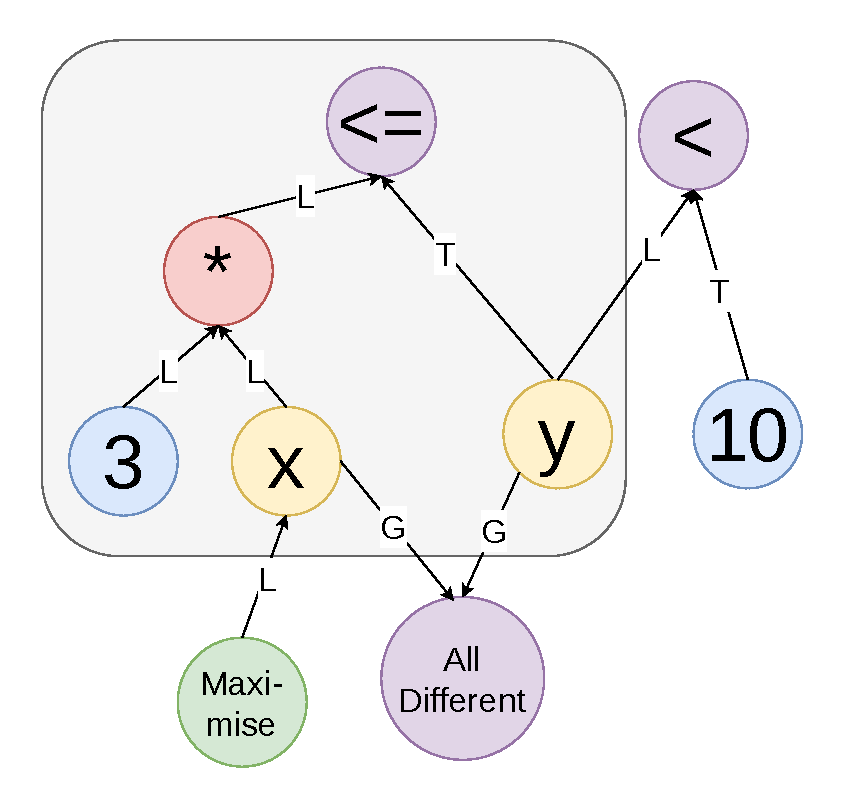
\includegraphics[width=.9\textwidth]{figures/graph.drawio.pdf}
    \end{subfigure}
    \caption{Conversion of a constraint model (left) to a graph (right). Variables in yellow, Parameters in blue, Operators in red, Constraints in purple, and Solve in green. The area in gray represents the constraint \texttt{3*x <= y}. Lead edges are labelled as L, Trailing as T and Global as G.}
    \label{fig:conversion}
\end{figure}

Figure \ref{fig:conversion} shows an example of how a simple constraint model can be converted using our conversion methodology.